\chapter{Aufwand}


Das Thema dieses Kapitels lässt sich mit einer Frage zusammenfassen:
Wie bemessen wir den Aufwand,
den es braucht ein Problem durch einen Algorithmus zu lösen?
In \autoref{einleitung} haben wir formale Sprachen als Repräsentation von Problemen eingeführt,
in \autoref{reg} haben wir gelernt, was ein Algorithmus ist und
in \autoref{turing} wurde eine Möglichkeit eingeführt,
alle bekannten Algorithmen zu implementieren:
die Turingmaschine.
Diesen Formalismus wollen wir in diesem Kapitel nutzen,
um genau zu spezifizieren,
was Aufwand bedeutet.

\section{Warum nicht einfach Messen?}\label{messenVsBeweisen}

Bevor wir uns dem Thema theoretisch nähern,
wollen wir noch eine ganz praktische Erwägung durchdenken:
Warum nicht einfach den Aufwand messen,
anstatt ihn über die Eigenschaften einer Turinmaschinen zu quantifizieren?
Die Idee hierbei:
Implementiere den Algorithmus in einer beliebigen Programmiersprache
und messe die Zeit,
wie lange die Implementierung läuft.
Hierbei ergeben sich einige Schwierigkeiten:
\begin{itemize}
  \item Auf welchem Input soll die Implementierung laufen?
      Die Menge der möglichen Inputs vieler Algorithmen ist unendlich,
      daher kann man nur Stichproben aus den möglichen Inputs nehmen
        und muss sich der Methodik der Statistik bedienen,
        um allgemeine Aussagen zu rechtfertigen.
    \item Das „Rauschen“ bei Messungen muss berücksichtigt werden:
        Die folgende Aufzählung von ``Störfaktoren'' machen
        die Vergleichbarkeit von Messergebnissen zu einer
        großen Herausforderung (die Liste ist wahrscheinlich nicht vollständig):
      \begin{itemize}
          \item Genutzte Hardware
          \item Genutztes Betriebssystem
          \item Spezifische Versionen (z.B. Compiler, Browser, OS)
          \item Lastsituation auf der Maschine
          \item Virtualisierung
          \item Netzauslastung
          \item Temperatur
          \item Messmethode
      \end{itemize}
\end{itemize}

Es ist also offensichtlich,
dass man nicht ``einfach'' messen kann.
Dennoch hat die empirische Messung auch in der Informatik ihren Platz.
Wir werden darauf noch einmal am Ende des Kapitels zurückkommen.

\subsection{Warum eine empirische Messung dennoch sinnvoll ist}
Die Idee den Aufwand eines Algorithmus über das ``Laufzeitverhalten'' einer Turingmaschine zu bestimmen,
umgeht die Herausforderungen empirischer Messungen, die wir am Anfang des Kapitels skizziert haben.

Eine Messung ist dennoch ein valides (wissenschaftliches) Instrument,
um Aussagen über Algorithmen und deren Implementierungen zu erhalten.
Der theoretische Ansatz dieses Kapitels basiert auf einigen Annahmen,
die selbst nicht unproblematisch sind:
\begin{itemize}
  \item Operationen haben auf einer Turingmaschine identischen Aufwand.
    Dies ist auf ``echter'' Hardware zumeist anders.
    Die Frage ist daher, welche Aussagekraft die Analyse eines Algorithmus auf einer Turingmaschine für realistische Szenarien hat.
  \item Daten und Zwischenergebnisse nutzen identischen Speicherplatz.
  \item Der Input einer Turingmaschine kann unendlich wachsen,
      In der Reailität ist dieser Platz begrenzt (z.B. der verfügbare Hauptspeicher).
  %\item Ist jeder Input gleich wahrscheinlich?
\end{itemize}

\section{Zeit-Aufwand}

Was meinen wir, wenn wir von Aufwand oder Effizienz einer Berechnung sprechen?
Meist wird als erstes die \emph{Zeit} genannt,
die es braucht,
damit eine Berechnung ein Ergebnis liefert.

Es wäre ebenso möglich,
den \emph{Speicherplatz} als Aufwandsdimension zu verstehen,
den eine Implementierung benötigt,
um den Input,
eventuelle Zwischenergebnisse
und den Output zu speichern.
Beides, Zeit und Speicherplatz sind valide Größen,
anhand derer wir Aufwand oder Effizienz bemessen können.
Wir werden uns in diesem Skript auf Zeit-Effizienz konzentrieren,
weswegen wir bei Aufwand beziehungsweise Effizienz immer von
zeitlichem Aufwand beziehungsweise zeitlicher Effizienz sprechen,
wenn wir Speicherplatz nicht explizit mitnennen.
Allerdings kann einiges auf Raum-Effizienz übertragen werden,
das wir in diesem Kapitel entwickeln.

Wir wollen über diese drei folgenden Schritte zu einem Verständnis von Aufwand kommen:
\begin{enumerate}
    \item Aufwand für einen einzelnen Lauf einer spezifischen Turingmaschine
    \item Aufwand für alle Läufe auf einer spezifischen Turingmaschine
    \item Schranken für alle Läufe auf allen Turingmaschinen,
        die eine spezifische Sprache erkennen, also ein spezifisches Problem lösen.
\end{enumerate}

Die folgenden Abschnitte folgen diesen Schritten,
indem zuerst theoretisch die Aufwandsquantifikation erschlossen wird
und diese dann an einem Beispiel praktische durchgespielt.

\subsection{Aufwand eines einzelnen Laufs}
Am Anfang unserer Überlegung haben wir diese zwei Komponenten:
\begin{itemize}
    \item Ein \emph{Wort $w \in L$}
    \item Einen Algorithmus,
        implementiert als \emph{Turingmaschine $tm \in TM$}.\footnote{%
            $TM$ bezeichnet die Menge aller Turingmaschinen.}
\end{itemize}
Gesucht ist eine Funktion $\tau: L \times TM \rightarrow \mathbb{N}$,
die für ein Wort $w \in L$ auf einer bestimmten Turingmaschine $tm \in TM$
den zeitlichen Aufwand in einer natürlichen Zahl ausdrückt.

Glücklicherweise haben wir in \autoref{turing} bereits ein Konzept eingeführt,
dass wir hierfür nutzen können:
Die Länge des Laufes von $w$ auf $tm$:
$\tau: \Sigma^* \times TM \rightarrow \mathbb{N}$ ist die Funktion,
die für ein Wort $w \in \Sigma^*$ den Zeitaufwand auf einer Turingmaschine TM angibt.
Wir legen fest:
\[
    \tau(w,tm) = |l_{w,tm}| - 1
\]
Für ein Wort $w \in L$ ergibt sich eine Folge von Schnappschüssen,
dessen Länge (weniger 1, denn der Startschnappschuss muss abgezogen werden)
der Anzahl an Schritten entspricht,
die eine Turingmaschine braucht,
um das Wort zu erkennen.

\subsubsection{Beispiel: Drehe 100 um}

Wir wollen $\tau$ an einem Beispiel erläutern.
Sei REVERSE das folgende Problem:
\begin{itemize}
    \item \textbf{Gegeben}: Ein beliebig langes Binärwort $w_b \in \Sigma^*$ mit $\Sigma = \{0,1\}$.
    \item \textbf{Gesucht}: Das Wort rückwärts.
\end{itemize}

Wäre also $w_b = 100$, dann wäre $w_b' = 001$ gesucht und damit $w = 100001 \in REVERSE$.
REVERSE ist daher eine formale Sprache,
welche die ``Rückwärts-Funktion'' kodiert:
REVERSE = $\{00, 11, 0000, 0110, 1001, 1111, \ldots\}$
\autoref{fig:tmreverse} zeigt eine Turingmaschine $tm_{REVERSE}$, die REVERSE erkennt.

Den konkreten Lauf auf $w_b = 100$ wollen wir nutzen,
um zu zeigen, wie sich der Wert von $\tau(w_b, tm_{REVERSE})$ feststellen lässt.

\newpage
\begin{figure}[H] % ’ht’ tells LaTeX to place the figure ’here’ or at the top of the page

\centering % centers the figure
\begin{tikzpicture}
    %Initial part
    \node[state, initial] (I) {I};
    \node[state, below of=I] (C) {C};
    %Loop part
    \node[state, below of=C] (LS) {LS};
    \node[state, below of=LS] (L0) {L0};
    \node[state, below left of=L0] (0L1) {0L1};
    \node[state, below right of=L0] (1L1) {1L1};
    \node[state, below of=0L1] (0L2) {0L2};
    \node[state, below of=1L1] (1L2) {1L2};
    \node[state, below right of=0L2] (L3) {L3};
    \node[state, below right of=1L2] (L4) {L4};

    %Finish part
    \node[state, right of=LS] (F0) {F0};
    \node[state, above right of=F0] (0F1) {0F1};
    \node[state, right of=0F1] (0F2) {0F2};
    \node[state, below right of=F0] (1F1) {1F1};
    \node[state, right of=1F1] (1F2) {1F2};
    \node[state, accepting, below right of=0F2] (F3) {F3};
	\draw

%        %Initial part
         (I) edge[left] 
            node[text width=1cm, align=center]{0,0,R\\1,1,R}
             (C)
         (C) edge[bend left=90, above] node{$\square$,$\square$,L} (F3)
         (C) edge[left] 
             node[text width=1cm, align=center]{0,0,R\\1,1,R}
             (LS)
%        %Loop part
         (LS) edge[above] node{$\square$,$\square$,L} (F0)
         (LS) edge[left] 
            node[text width=1cm, align=center]{0,0,L\\1,1,L}
            (L0)
         (L0) edge[above right] node{1,$\square$,L} (1L1)
         (L0) edge[above left] node{0,$\square$,L} (0L1)

         (0L1) edge[loop left] 
            node{$\square$,$\square$,L}
            (0L1)
         (0L1) edge[left] 
             node[text width=1cm, align=center]{0,0,L\\1,1,L}
             (0L2)
         (0L2) edge[loop left] 
            node[text width=1cm, align=center]{0,0,L\\1,1,L}
            (0L2)
         (0L2) edge[left] node{$\square$,0,R} (L3)

         (1L1) edge[loop left] 
            node{$\square$,$\square$,L}
            (1L1)
         (1L1) edge[left] 
             node[text width=1cm, align=center]{0,0,L\\1,1,L}
             (1L2)
         (1L2) edge[loop left] 
            node[text width=1cm, align=center]{0,0,L\\1,1,L}
            (1L2)
         (1L2) edge[right] node{$\square$,1,R} (L3)

         (L3) edge[loop below] 
            node[text width=1cm, align=center]{0,0,R\\1,1,R}
             (L3)
         (L3) edge[above] node{$\square$,$\square$,R} (L4)

         (L4) edge[loop below] 
            node{$\square$,$\square$,R}
         (L4)
         (L4) edge[bend right=20, right] 
            node[text width=1cm, align=center]{0,0,R\\1,1,R}
         (LS)
%        %Finish part
         (F0) edge[above left] node{0,$\square$,L} (0F1)
         (0F1) edge[loop below] 
            node{$\square$,$\square$,L}
            (0F1)
         (0F1) edge[above] 
            node[text width=1cm, align=center]{0,0,L\\1,1,L}
            (0F2)
         (0F2) edge[loop below] 
            node[text width=1cm, align=center]{0,0,L\\1,1,L}
            (0F2)
         (0F2) edge[above right] node{$\square$,0,-} (F3)

         (F0) edge[below left] node{1,$\square$,L} (1F1)
         (1F1) edge[loop below] 
            node{$\square$,$\square$,L}
            (1F1)
         (1F1) edge[above] 
            node[text width=1cm, align=center]{0,0,L\\1,1,L}
            (1F2)
         (1F2) edge[loop below] 
            node[text width=1cm, align=center]{0,0,L\\1,1,L}
            (1F2)
         (1F2) edge[below right] node{$\square$,1,-} (F3)

    ;
\end{tikzpicture}
\caption{$tm_{REVERSE}$}%
\label{fig:tmreverse}
\end{figure}

\newpage
Dies ist der Lauf $l_{10, tm_{REVERSE}}$:

\setcounter{arraycounter}{-1}
\begin{center}
$
\arraycolsep=15.0pt
    \begin{array}{>{\stepcounter{arraycounter}\thearraycounter\mspace{20mu}}llrlrl}
[   & [I,   & \sq,          & 1,    & 00]               & , \\
    & [C,   & \sq1,         & 0,    & 0]                & , \\
    & [LS,  & \sq10,        & 0,    & \sq]              & , \\
    & [L0,  & \sq1,         & 0,    & 0\sq]             & , \\
    & [0L1, & \sq,          & 1,    & \sq0\sq]          & , \\
    & [0L2, & \sq,          & \sq,  & 1\sq0\sq]         & , \\
    & [L3,  & \sq0,         & 1,    & \sq0\sq]          & , \\
    & [L4,  & \sq01,        & \sq,  & 0\sq]             & , \\
    & [L4,  & \sq01\sq,     & 0,    & \sq]              & , \\
    & [LS,  & \sq01\sq0,    & \sq,  & \sq]              & , \\
    & [F0,  & \sq01\sq,     & 0,    & \sq\sq]           & , \\
    & [0F1, & \sq01,        & \sq,  & \sq\sq\sq]        & , \\
    & [0F1, & \sq0,         & 1,    & \sq\sq\sq\sq]     & , \\
    & [0F2, & \sq,          & 0,    & 1\sq\sq\sq\sq]    & , \\
    & [0F2, & \sq,          & \sq,  & 01\sq\sq\sq\sq]   & , \\
    & [F3, & \sq,           & 0,    & 01\sq\sq\sq\sq]   & ] \\
\end{array}
$
\end{center}

Da $|l_{100,tm_{REVERSE}}| = 16$ hat $\tau$ in diesem Fall also den folgenden Wert:
\[
\tau(100,tm) = 15
\]

\subsection{Aufwandsquantifikation für eine Implementierung}

Bisher haben wir aber nur über den Aufwand gesprochen,
den ein spezifischer Lauf auf einem Wort verursacht,
nicht aber,
wie sich der Aufwand für eine komplette Implementierung quantifizieren lässt.
Wir betrachten daher also:
\begin{itemize}
    \item Die konkrete Implementierung eines Algorithmus,
        gegeben als \emph{Turingmaschine $tm \in TM$}.
\end{itemize}

Wie können wir nun auf den Ergebnissen aus dem vorherigen Abschnitt aufbauen?
Eine Sprache kann unendlich viele Worte enthalten,
d.h. Lösungen, die darauf beruhen,
dass es ein Minimum oder Maximum von $\tau$ für ein Wort $w \in L$ gibt,
sind nicht zielführend.

Wir können aber die \emph{Größe} des Inputs in Relation zum Aufwand setzen,
und so die Implementierung charakterisieren.
Um zu beschreiben,
wie groß der Aufwand für eine Implementierung ist,
suchen wir daher eine Funktion,
welche die Inputgröße auf Anzahl der Schritte abbildet,
die eine Implementierung benötigt,
um das Problem zu lösen.
Übertragen auf den Kontext der formalen Sprachen und Turingmaschinen
können wir die Wortlänge betrachten:
Beschreibe, wie sich das Laufzeitverhalten einer Turingmaschine
bei wachsender Wortlänge verhält.
%TODO Grafik

Gesucht ist also die folgende Funktion:
$t: \mathbb{N} \times TM \rightarrow \mathbb{N}$,
also die Abbildung einer Wortlänge und einer Turingmaschine
auf die Anzahl der Schritte für ein Wort dieser Länge.
Da mehrere Worte die gleiche Länge haben können,
müssen wir die Möglichkeiten diskutieren,
wie wir in diesem Falle zu einem eindeutigen Wert kommen können:
\begin{itemize}
    \item \textbf{Best Case}: Wir wählen das Wort der Länge aus,
        für das der Algorithmus den kürzesten Lauf hat,
        also die geringste Zeit benötigt.
    \item \textbf{Average Case}: Wir nutzen statistische Methoden,
        um die wahrscheinliche Länge eines Laufs zu quantifizieren.
        Wir betrachten also zum Beispiel den Erwartungswert von $\tau$,\footnote{%
            In diesem Fall bildet $tm$ auf $\mathbb{Q}$ ab und nicht mehr auf $\mathbb{N}$.}
        wenn wir per Zufall ein Wort aus L der gegebenen Länge auswählen.\footnote{%
            Der Modus (entspricht dem Median in einer endlichen Stichprobe) wäre eine Alternative.
        Mit der Standardabweichung (Streuungsmaß) oder einer Kombination mehrerer Maße,
        verbessert sich die Aussagekraft,
        was aber die einfache Vergleichbarkeit von Algorithmen wiederum erschwert.}

    \item \textbf{Worst Case}: Wir wählen das Wort aus,
        für das der Algorithmus den längsten Lauf hat,
        also die meiste Zeit benötigt.
\end{itemize}

Da der Best Case meist wenig Aussagekraft über die Güte des Algorithmus besitzt,
wird er selten als Maß für den Aufwand eines Problems genutzt.
Am aussagekräftigsten ist der Average Case,
aber um ihn formal sauber anzuwenden braucht es
entsprechendes statistisches Werkzeug.\footnote{%
    Für interessierte Leser:innen sei~\cite{knuth1}, 96ff bzw. 1.2.10 empfohlen,
    hier spielt Knuth die probabilistische Analyse des Euklidischen Algorithmus durch.}
Ganz pragmatisch konzentrieren wir uns auf Weiteres auf den Worst Case,
wenn wir nichts Anderslautendes angeben.


$t$ können wir mit diesen Überlegungen also definieren als:
\[
t(n, tm) = \max({\tau(w, tm)| |w| = n})
\]
$t$ gibt also die jeweilige Worst Case Laufzeit für ein Wort der Länge $n$ an.
Dies erlaubt es uns auch über unendlich große formale Sprachen Aussagen zu treffen,
indem wir angeben,
wie sich der Aufwand bei steigender Inputgröße,
also bei steigender Wortlänge, entwickelt.

Wir wollen nun noch eine Blaupause geben,
wie wir viele Turingmaschinen,
bezüglich Ihres Aufwandsverhalten analysiseren können:
\begin{enumerate}
    \item Identifiziere alle Basispfade.\footnote{%
            Basispfade sind die kürzestenPfade vom Startzustand in einen Endzustand}
    \item Lege symmetrische Pfade zusammen.\footnote{%
            Symmetrische Pfade sind solche,
            die identisch viele Schritte brauchen und an identische Orte,
            identisch viele Zeichen schreiben.}
    \item Zähle die Schritte der schleifenlosen Pfade.
    \item Zähle die Schritte der schleifenlosen Teilpfade von Schleifenpfaden.
    \item Für die Teilpfade, die nur EinerSchleifen\footnote{%
            Einerschleifen sind Schleifen die nur über einen Zustand gehen (Loops in den Grafiken)},
        quantifiziere den Aufwand als Funktion, basierend auf einem Restwortmodell.
    \item Für die Teilpfade mit komplexen Schleifen,\footnote{%
            Komplexe Schleifen sind Schleifen, die über mehr als einen Zustand gehen.}
            wende das Verfahren ab Schritt 1
        rekursiv auf die Teilpfade an, mit Startzustand beim Schleifeneingang
        und Endzustand beim Schleifenausgang.
    \item Zähle alle Schritte zusammen, bis alle Basispfade quantifiziert sind.
    \item Identifiziere die Logik, auf welchem Pfad der Worstcase für n liegt.
    \item Gib die Funktion $t$ an.
\end{enumerate}
Dieses Verfahren ist in der Tat nur eine Blaupause,
das wir es nicht in einen Algorithmus verwandeln können:
Wir wissen nicht, ob das Verfahren für jede Turingmaschine endet.\footnote{%
    Genaueres über die Gründe werden wir in \autoref{derBarbierUndDerLuegner} erfahren.}

\subsubsection{Beispiel: Aufwand für $tm_{REVERSE}$}

Für $tm_{REVERSE}$ können wir zwei Basispfade identifizieren:
\begin{enumerate}
        \item Für Worte $w$ mit $|w| = 1$: I $\rightarrow$ C $\rightarrow$ F3.\\
            Die Schrittanzahl hier ist 2.
        \item Für Worte $w$ mit $|w| > 1$ gibt es zwei symmetrische Basispfade:\\
            I $\rightarrow$ C $\rightarrow$ LS $\rightarrow$ FO $\rightarrow$ OF1/1F1 $\rightarrow$ 0F2/1F2 $\rightarrow$ F3.\\
            Die folgenden Teilpfade sind auszumachen:
            \begin{enumerate}
                \item Die Schrittanzahl für den ersten schleifenlosen Part I $\rightarrow$ C $\rightarrow$ LS ist 2.\\
                \item Wir haben einen Teilpfad $LS$ mit einer komplexen Schleife, deren Funktion wir mit x bezeichnen,
                    wir wenden die Methode rekursiv auf x an mit LS als Start und Ende der komplexen Schleife.
                \item Für den Teilpfad F0 $\rightarrow \ldots \rightarrow$ F3 haben wir nur Einerschleifen,
                    deren Funktion wir mit y bezeichen (siehe Restwortemodell 1).
            \end{enumerate}
\end{enumerate}

Da Worte gleicher Länge auch gleich lange Läufe auf $tm_{REVERSE}$ haben
(da, wo sich die Läufe qua Zeichen unterscheiden,
sind die parallelen Pfade in $tm_{REVERSE}$ \emph{symmetrisch}).

Daraus ergibt sich die folgende Funktionsdefinition:
\[
    t(n, tm) = \begin{cases}
        2\text{, wenn } x = 1,\\
        2 + x(n) + y(n) \text{, wenn } x > 1,\\
    \end{cases}
\]
            
Für $x(n)$ lässt sich feststellen, dass die Pfade in der Schleife symmetrisch sind.
Anhand von \autoref{fig:x_wm} lässt sich das Restwortmodell so einführen.
$c_i$ mit $2 \leq i < n$ ist der Index, des zu kopierenden Zeichen.
Wir starten auf dem Zeichen rechts von $c_i$ (damit wissen wir,
dass wir danach noch mindestens ein weiteres Zeichen kopieren müssen).
Wir gehen einen Schritt nach links,
dann $(i-1)$ Schritte nach links, bis wir bei $c_1/c^{'}_{n}$ angelangt sind.
Dann weitere $(i-1)$ Schritte nach links, bis wir an dem Punkt sind, an dem
wir $c^{'}_{n-i}$ einsetzen.
Die gleiche Schrittanzahl ($2i -1$) gehen wir wieder zurück und dann noch zwei Schritte.
Daher ergibt sich für jedes zu kopierende Zeichen $i$ die Schrittanzahl $4i - 1$.
Für alle Schritte zusammen (wir wiederholen das ganze n-2 mal) ergibt sich daher:

\begin{figure}[hb]
    \caption{Restwortmodell für $x(n)$}
    \centering
    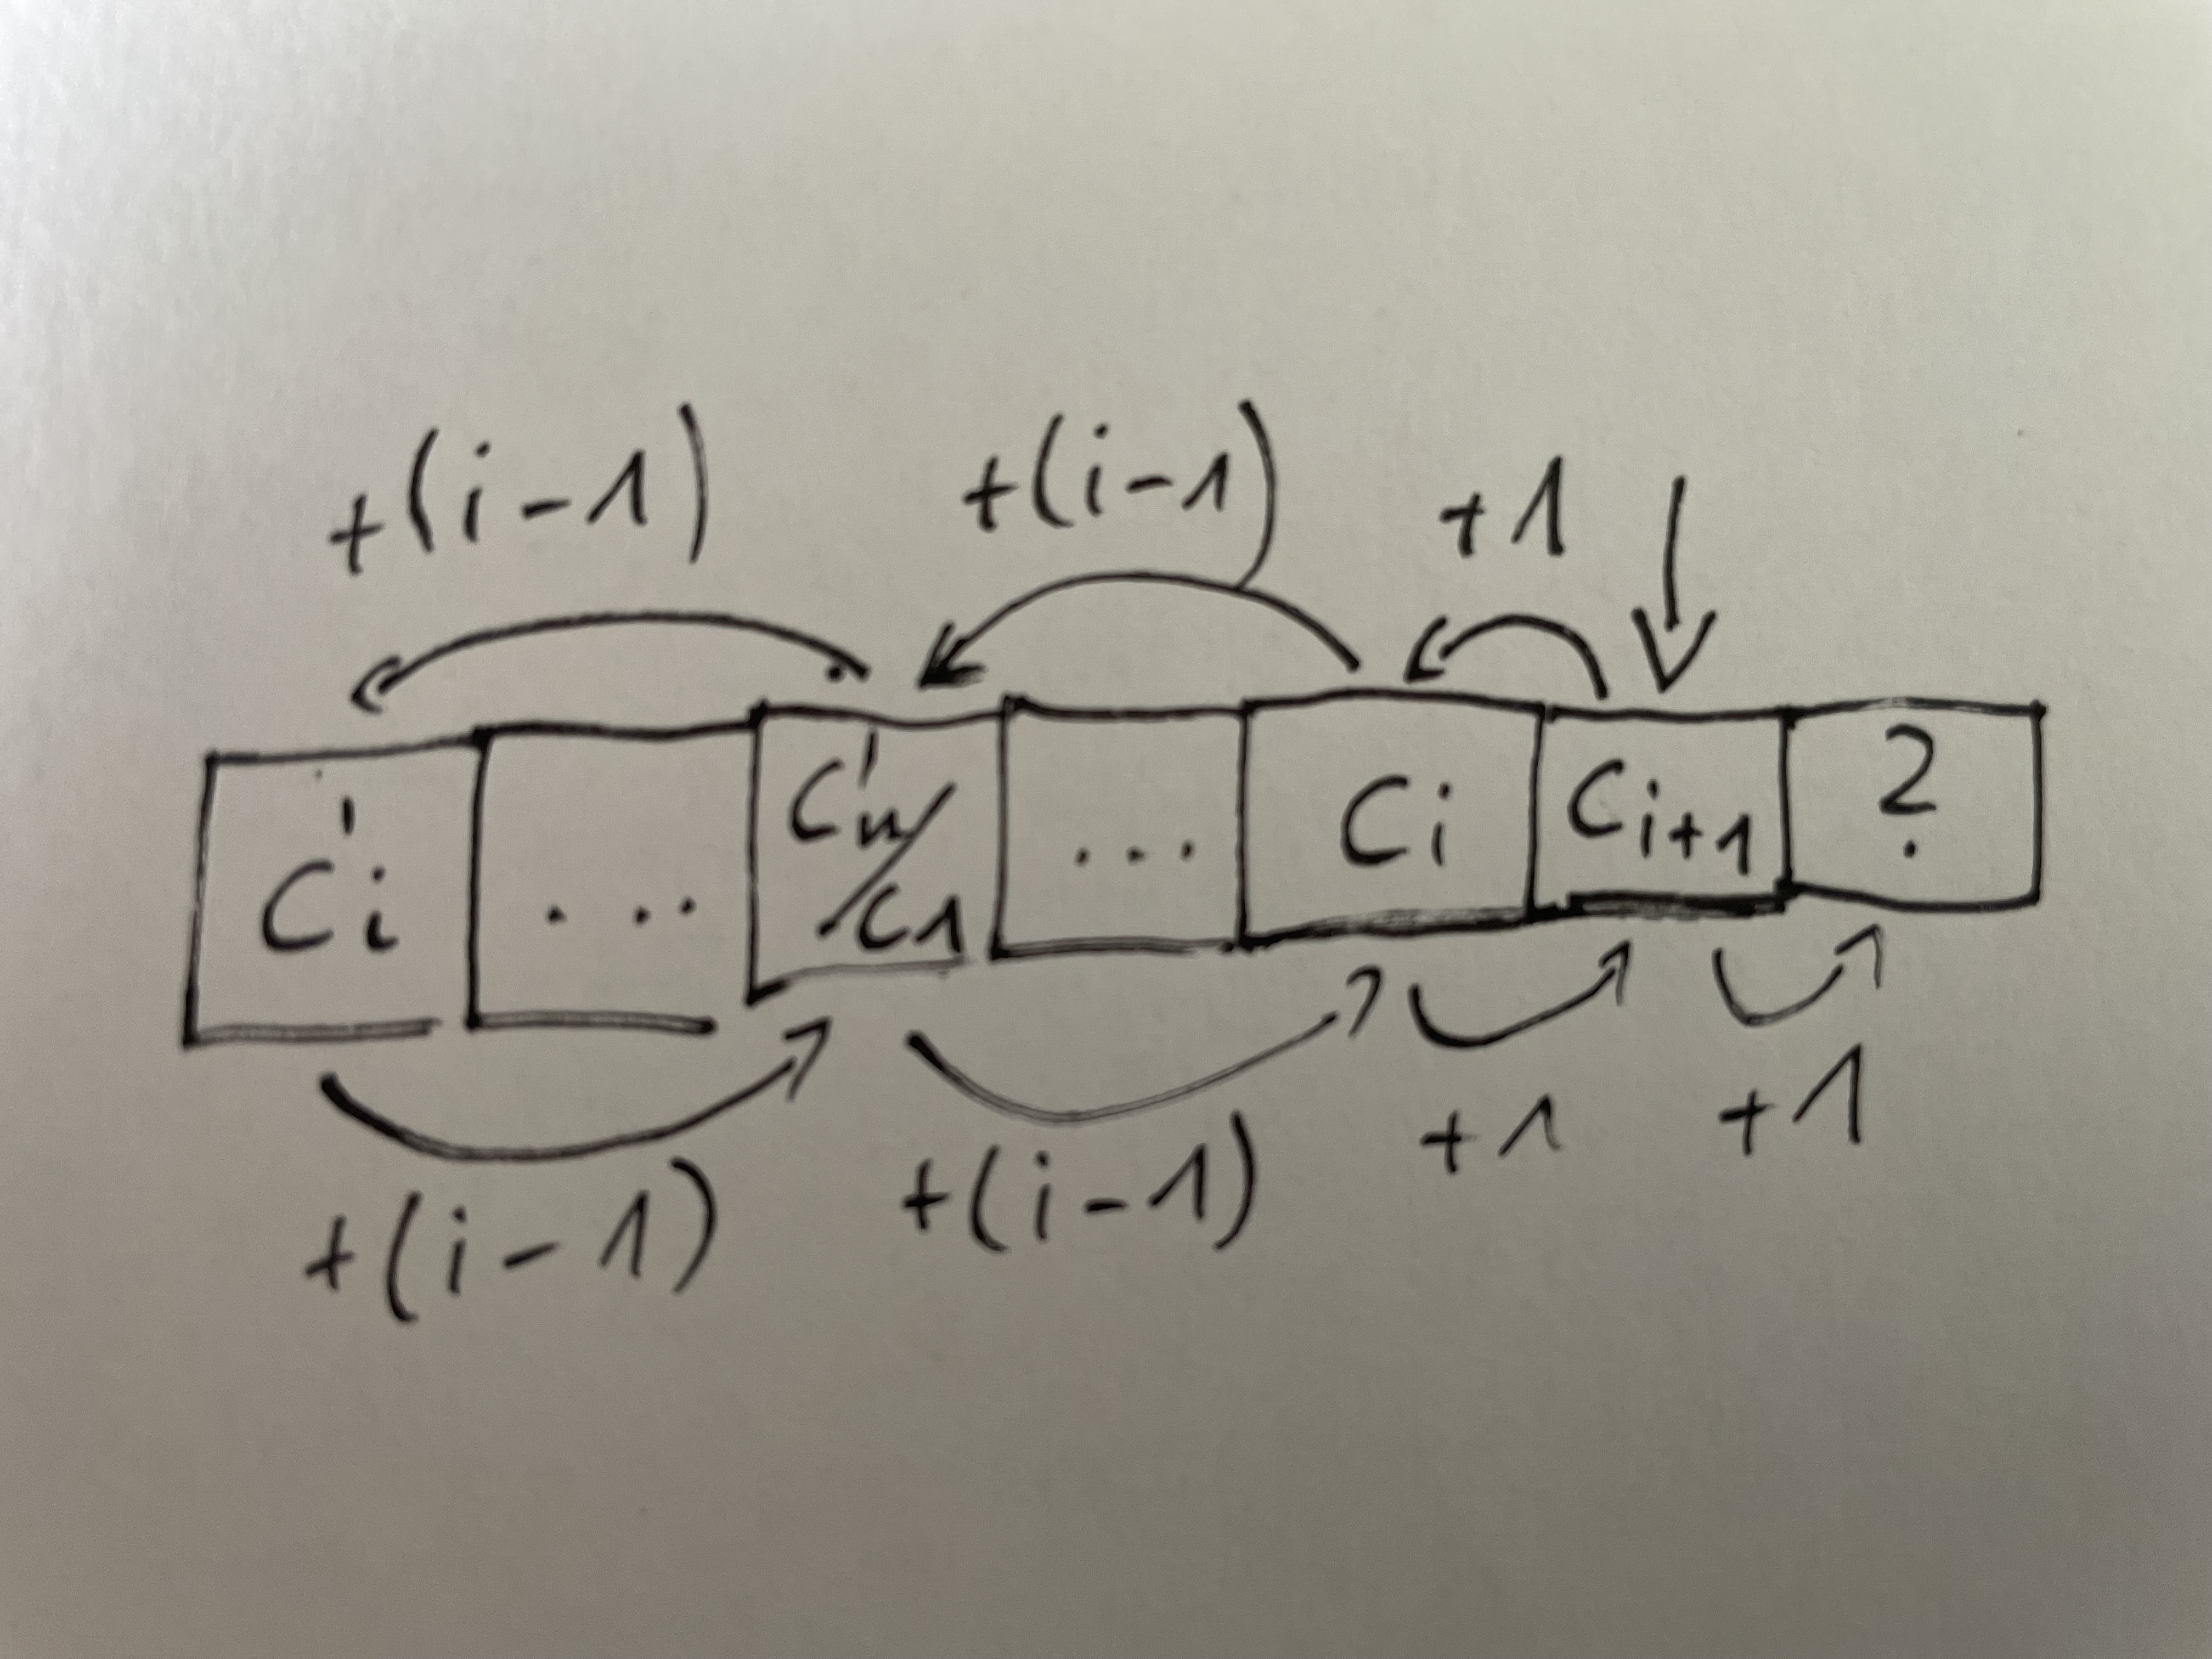
\includegraphics[width=0.5\textwidth]{x_kap4}%
    \label{fig:x_wm}
\end{figure}



\begin{align*}
    x(n) &=&                &   & \sum_{i=2}^{n-1} 4i - 1     &            \\ 
         &=& -(4 - 1)       & + & (\sum_{i=1}^{n} 4i -1)      & - (4n - 1) \\
         &=& -3             & + & -n + 4 (\sum_{i=1}^{n} i)   &  - 4n + 1  \\
         &=& -5n -2         & + & 4 (\frac{n^2+n}{2})         &            \\
         &=& -5n -2         & + & 2 n^2 + 2n                  &            \\
         &=& 2n^2 -3n -2    &   &                             &            
\end{align*}


\begin{figure}[hb]
    \caption{Restwortmodell für $y(n)$}
    \centering
    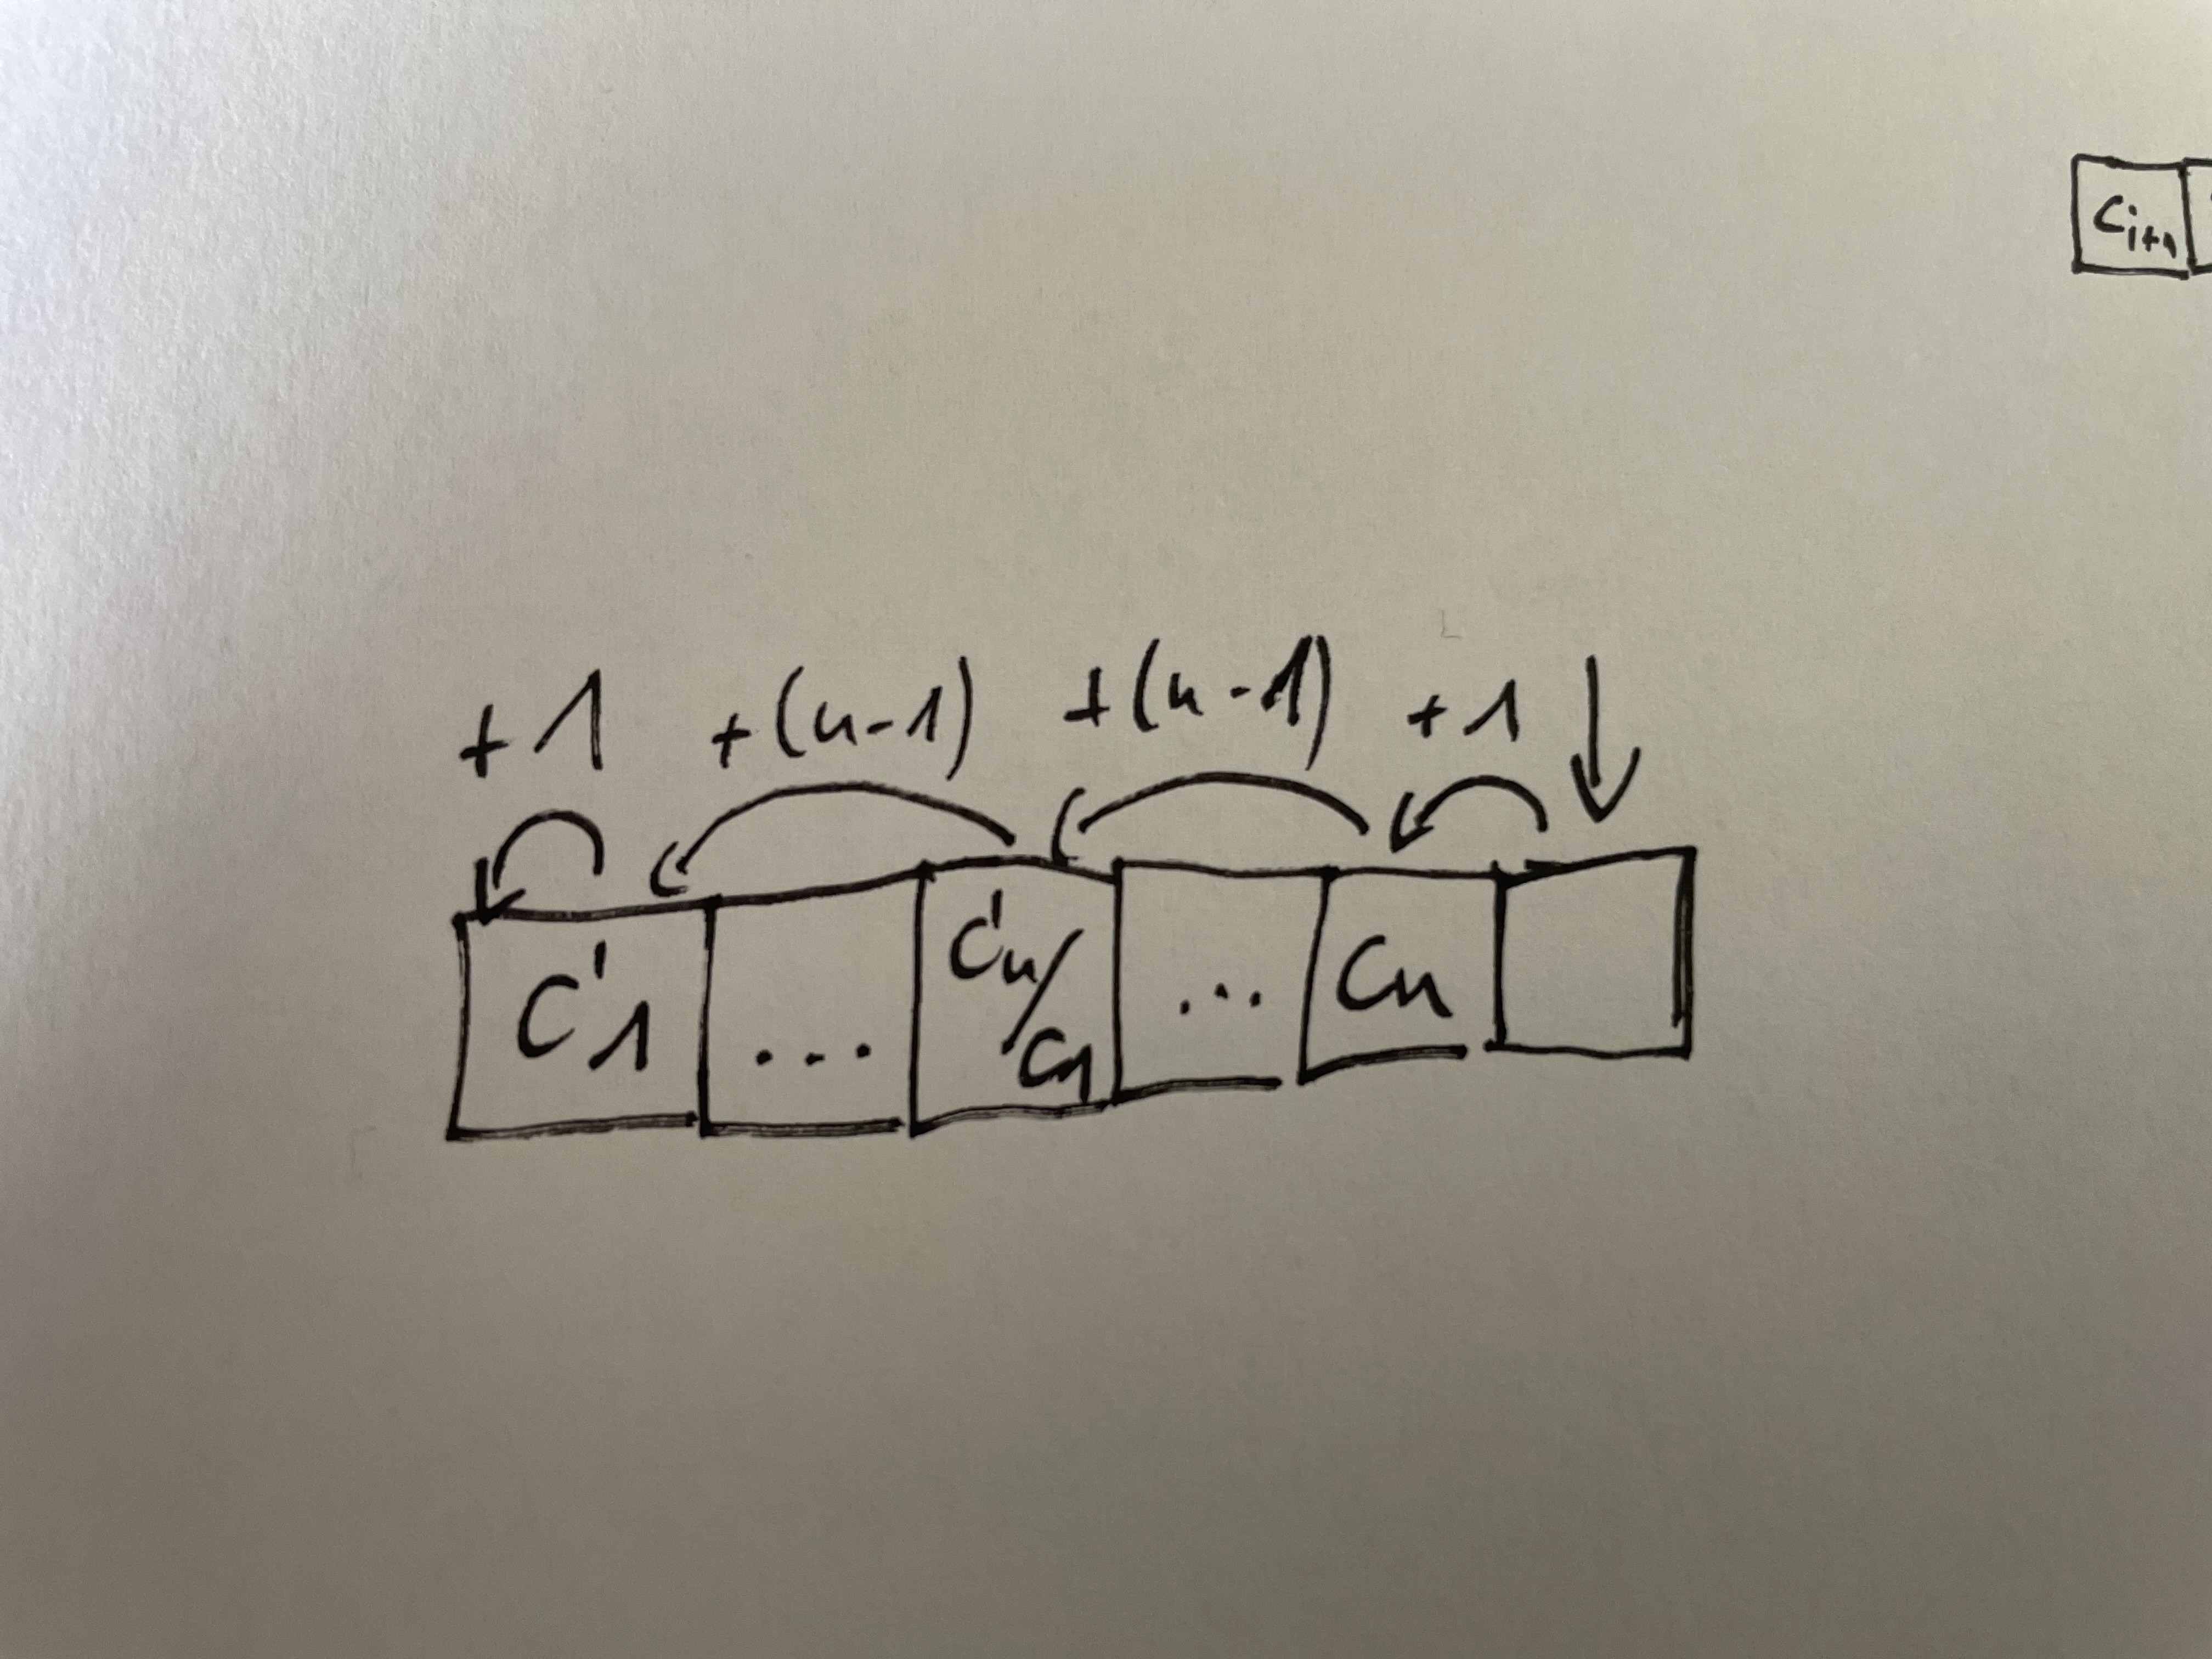
\includegraphics[width=0.5\textwidth]{y_kap4}%
    \label{fig:y_wm}
\end{figure}
Mit \autoref{fig:y_wm} ergibt sich $y(n) = 2n$.
Daher können wir die finale Definition von $t(n, tm)$ festhalten:
\[
    t(n, tm) = \begin{cases}
        2\text{, wenn } x = 1,\\
        2 n^2 -n \text{, wenn } x > 1,\\
    \end{cases}
\]

Um unsere Definition zu überprüfen, messen wir die Länge der Läufe für  $1 \leq i \leq 5$
(siehe \autoref{tab:ttmreverse}).
Die Funktionsdefinition wird also bestätigt.
\begin{table}[ht]
    \caption{$t(i,tm_{REVERSE})$ für $1 \leq i \leq 5$}
    \centering
    \begin{tabular}{c c c c c c}
    \toprule
          i
        & 1
        & 2
        & 3
        & 4
        & 5
        \\
        \midrule
          $t(i,tm_{REVERSE})$
        & 2
        & 6
        & 15
        & 28
        & 45
        \\
    \bottomrule
    \end{tabular}%
    \label{tab:ttmreverse}
\end{table}


\subsection{Aufwand für ein Problem}
Mit $t_{tm}$ und dem Worst Case-Wert können wir Aussagen über den Aufwand treffen,
den ein bestimmter Algorithmus für ein bestimmtes Problem verursacht.
Wir treffen allerdings keine Aussagen darüber,
wie viel Aufwand das Problem \emph{an sich} erzeugt.
Dazu müssten wir Aussagen über alle prinzipiell \emph{möglichen} Algorithmen,
die das Problem lösen:
Den Aufwand eines Problems würden wir dann mit dem effizientesten Algorithmus gleichsetzen.
Oftmals ist der Nachweis nicht trivial,
ob ein Algorithmus nun der effizienteste für ein Problem gibt

Für REVERSE und Turingmaschinen scheint es keinen Algorithmus zu geben,
der schneller ist, als der in den Beispielen vorgestellte.
Skizzenhaft könnte ein Beweis wie folgt aussehen:
\begin{enumerate}
        \item Wir müssen in jedem Fall jedes Zeichen des Inputworts lesen.
        \item Bis auf ein Zeichen müssen wir jedes an die richtige Stelle verschieben.
        \item Damit müssen wir mindestens $(n-1)$ mal im Durschnitt $2n$ mal
            zwischen Eingabe und Ausgabe hin- und herwechseln.
        \item Daraus folgt, dass jeder Algorithmus mindestens $n^2 - n$ Schritte braucht.
\end{enumerate}

Den aktuellen Stand der Forschung für eine Reihe von relevanten Problemen
(z.B. Sortierung oder Suche) erlernt man in Vorlesungen über
Algorithmen und Datenstrukturen.



\section{Aufwand und Berechnungsmodel}
% Diskussion Modell TM (Einfachheit vs Realitätsnähe)
Skizze:
\begin{itemize}
        \item Revisiting REVERSE:\@ Kontraintuitiver Aufwand bei TMs
        \item Beispiel: Beschleunigung durch 2-Band-Maschine
        \item Simulation weiterer Berechnungsmethoden
        \item Warum doch 1-Band-TMs: Einfachheit
\end{itemize}

Warum nutzen wir (in diesem Skript) Turingmaschinen zur Aufwandsquantifikation?
Wir haben die Church-Turing-These eingeführt und operieren auf der Annahme,
dass sich jedes (berechenbare) Problem durch eine Turingmaschine lösen lässt.

Andere Formalismen lassen sich auf einer Turingmaschine simulieren und
der Aufwand der Simulation lässt sich quantifizieren,
so wir können die ``Beschleunigigung'' durch andere Formalismen
(z.B. solche, die einen realistisches Speicherkonzept haben)
genau beziffern.

\begin{itemize}
    \item Relativ zur Implementierungssprache (Mehrbandturingmaschinen, Registermaschinen)
    \item Relativ zur Datenrepräsentation (Größe des Alphabets, Art der Datenstrukturen)
\end{itemize}

\section{Landau und Big-O:\@ Wachstum}

$t_{tm}$ ist eine Möglichkeit,
die Aufwandsentwicklung für steigende Inputgrößen formal zu spezifizieren.
Für die meisten Fälle ist $t_{tm}$ aber zu feingranular:
Wir interessieren uns beispielsweise nur dafür,
ob sich das Laufzeitverhalten sinnvoll beschränken lässt,
also ob es eine asymptotische obere oder untere Schranke für den Aufwand gibt.

Dies wird typischerweise mit der Landau-Notation angeben.
Wir definieren eine Menge von Funktionen in Abhängigkeit einer oberen Schranke
und lassen dabei Faktoren außen vor,
die für die Wachstumsdynamik unwesentlich sind:

\[
O(g(n)) = \{f|\exists c \exists n_0 \forall n (n \geq n_0 \rightarrow f(n) \leq c \cdot g(n))\}
\]
% TODO: Ergänze andere Klassen (o, $\theta$ usw).

\subsection*{Aufgaben}

\begin{enumerate}
    \item Gegeben sei die Turingmaschine $tm_{REVERSE2}$ (\autoref{fig:tmreverse2}) für die gilt: $L(tm_{REVERSE}) = L(tm_{REVERSE2})$.
            \begin{enumerate}
                \item Gib Länge $\tau(i, tm_{REVERSE2})$ mit $1 \leq i \leq 5$ an.
                \item Leite analog zu Kapitel x $t(n, tm_{REVERSE2})$ ab.
                \item Gilt $t \in O(t_{a})$?
            \end{enumerate}
\end{enumerate}

\begin{figure}[H] % ’ht’ tells LaTeX to place the figure ’here’ or at the top of the page
\centering % centers the figure
\begin{tikzpicture}
    %Initial part
    \node[state] (zLI) {$z_{LI}$};
    \node[state, left of=zLI] (zI12) {$z_{I12}$};
    \node[state, above of=zLI] (zI02) {$z_{I02}$};
    \node[state, above of=zI12] (zI11) {$z_{I11}$};
    \node[state, above of=zI02] (zI01) {$z_{I01}$};
	\node[state, initial, left of=zI01] (zI) {$z_I$};

    %Loop part
    \node[state, right of=zLI] (zL01) {$z_{L01}$};
    \node[state, above right of=zL01] (zLC) {$z_{LC}$};


    \node[state, below of=zL01] (zL02) {$z_{L02}$};

    \node[state, below right of=zLC] (zL11) {$z_{L11}$};
    \node[state, below of=zL11] (zL12) {$z_{L12}$};

    \node[state, below left of=zL12] (zL3) {$z_{L3}$};

    %Finish part

    \node[state, above left of=zLC] (zF0) {$z_{F0}$};
    \node[state, above right of=zF0] (zF1) {$z_{F1}$};
    \node[state, accepting, right of=zF1] (zF2) {$z_{F2}$};

	\draw

        %Initial part
        (zI) edge[above] node{0,0,L} (zI01)
        (zI01) edge[right] node{$\square$,$\square$,L} (zI02)
        (zI02) edge[left] node{$\square$,0,R} (zLI)

        (zI) edge[above right] node{1,1,L} (zI11)
        (zI11) edge[left, right] node{$\square$,$\square$,L} (zI12)
        (zI12) edge[above] node{$\square$,1,R} (zLI)

        %Loop part
        (zLC) edge[left] node{0,0,L} (zL01)
        (zLC) edge[above right] node{1,1,L} (zL11)
        (zLC) edge[right] node{$\square$,$\square$,L} (zF0)

        (zL01) edge[loop right] node{$\square$,$\square$,L} (zL01)
        (zL01) edge[left]
            node[text width=1cm, align=center]{0,0,L\\1,1,L}
            (zL02)

        (zL02) edge[loop right]
            node[text width=1cm, align=center]{0,0,L\\1,1,L}
            (zL02)
        (zL02) edge[right] node{$\square$,0,R} (zL3)

        (zL11) edge[loop right] node{$\square$,$\square$,L} (zL11)
        (zL11) edge[left]
            node[text width=1cm, align=center]{0,0,L\\1,1,L}
            (zL12)

        (zL12) edge[loop right]
            node[text width=1cm, align=center]{0,0,L\\1,1,L}
            (zL12)
        (zL12) edge[right] node{$\square$,1,R} (zL3)


        (zL3) edge[loop below]
            node[text width=1cm, align=center]{0,0,R\\1,1,R}
            (zL3)
        (zL3) edge[bend left, left] node{$\square$,$\square$,R}(zLI)

        (zLI) edge[in=210, out=240, looseness=8, below] node{$\square$,$\square$,R} (zLI)
        (zLI) edge[bend left, above left]
            node[text width=1cm, align=center]
            {0,$\square$,R\\1,$\square$,R}
            (zLC)

        %Finish part
        (zF0) edge[loop above] node{$\square$,$\square$,L} (zF0)
        (zF0) edge[below right]
            node[text width=1cm, align=center]{0,0,L\\1,1,L}
            (zF1)
        (zF1) edge[loop above]
            node[text width=1cm, align=center]{0,0,L\\1,1,L}
            (zF1)
        (zF1) edge[above] node{$\square$,$\square$,R} (zF2)
    ;
\end{tikzpicture}
\caption{$tm_{REVERSE2}$}%
\label{fig:tmreverse2}
\end{figure}
